\section{Конструкторская часть}

В этом разделе представлена архитектура разработанного протокола. Описаны используемые структуры данных.

\subsection{Архитектура протокола}

\subsubsection{Описание протокола}

На рисунке \ref{fig:proto_scheme} представлена концептуальная схема работы протокола.

\begin{figure}[H]
	\centering
	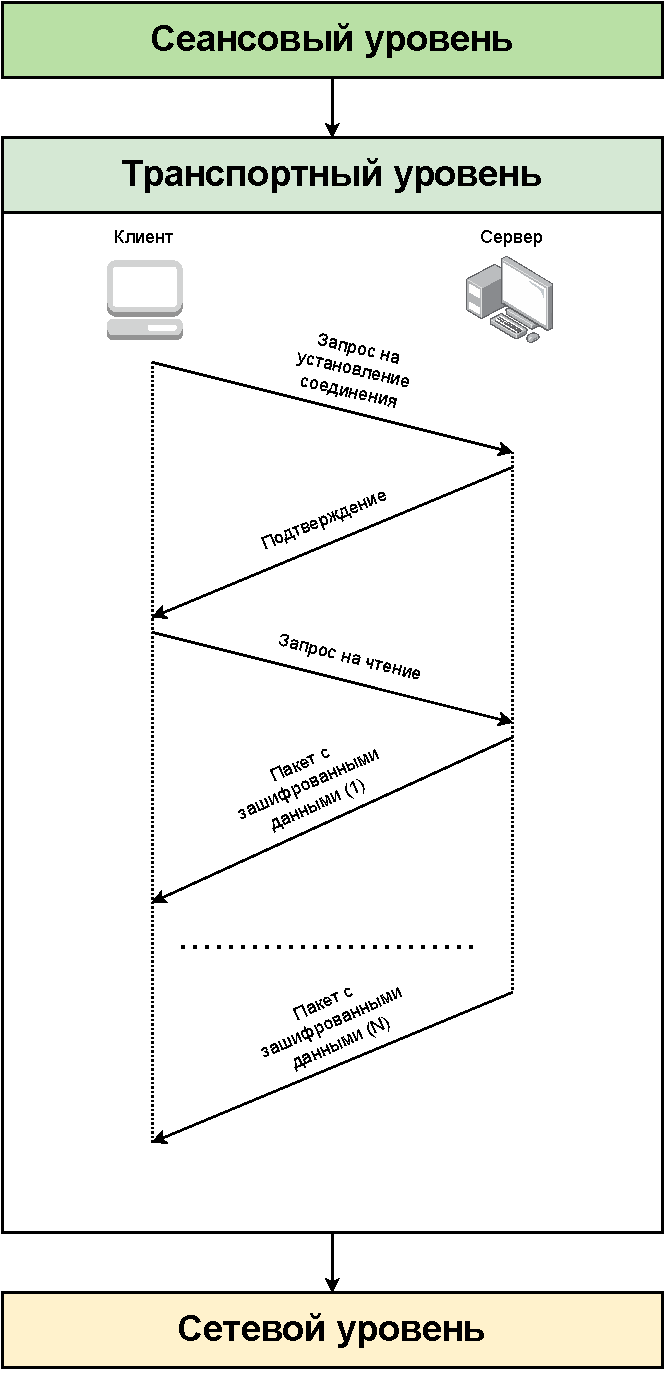
\includegraphics[scale=0.75]{img/proto_scheme.pdf}
	\caption{Концептуальная схема работы протокола}
	\label{fig:proto_scheme}
\end{figure}

Шаги работы протокола можно описать следующим образом:

\begin{enumerate}
	\item клиент отправляет серверу запрос на установления соединения;
	\item сервер отправляет ответ-подтверждение;
	\item если подтверждение на установление соединения не получено, клиент завершает свою работу;
	\item в случае, если подтверждение получено, клиент отправляет запрос на чтение данных;
	\item сервер подготавливает пакеты к отправке, предварительно зашифровывая передаваемые данные;
	\item сервер отправляет клиенту пакеты с зашифрованными данными;
	\item клиент расшифровывает полученные от сервера данные;
\end{enumerate}

Размер передаваемых данных должен обязательно кратен блоку шифрования. В обратном случае, сервер дополняет их необходимым количеством байт, состоящим из нулей.

\subsubsection{Шифрование данных}

Для шифрования данных используется симметричный алгоритм AES-192. Это означает, что один и тот же ключ используется и для шифрования, и для расшифровки отправляемых данных. Протокол предполагает, что ключ не передаётся по сети. Сервер и клиент должны самостоятельно определить, какой ключ шифрования необходимо использовать для шифрования и расшифровывания данных.

\subsection{Структура пакета}

\subsubsection{Описание пакета}

Пакет, используемый в проектируемом протоколе, можно разделить на три логических части:

\begin{enumerate}
	\item заголовок IP -- метаданные, необходимые для сетевого уровня OSI.
	\item метаданные пакета  -- информация о передаваемых данных;
	\item полезная нагрузка -- непосредственно сами данные.
\end{enumerate}

Описание структуры пакета представлено на рисунке \ref{fig:packet}.

\begin{figure}[H]
	\centering
	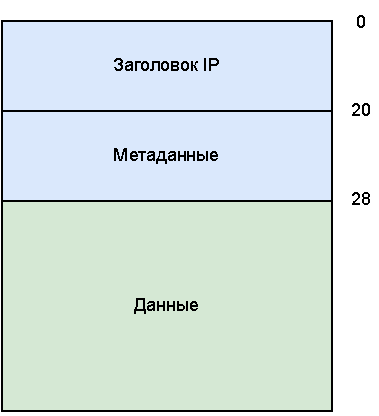
\includegraphics[width=\textwidth]{img/packet.pdf}
	\caption{Структура пакета}
	\label{fig:packet}
\end{figure}

Под заголовок IP выделяется первые 20 байт, а для метаданных следующие восемь байт. Остальная память используется для хранения данных, размер которые не может превышать 65488 байт и должен быть кратен размеру блоку шифрования (16 байт). Зашифрованными передаются только сами данные, содержимое IP заголовка и метаданных передается в не зашифрованном виде.

Для каждого отправляемого пакета вычисляется контрольная сумма, которая является суммой хэш-сумм IP-заголовка, метаданных и данных (в зашифрованном виде).

\subsubsection{Метаданные}

На рисунке \ref{fig:header} представлено описание метаданных пакета.

\begin{figure}[H]
	\centering
	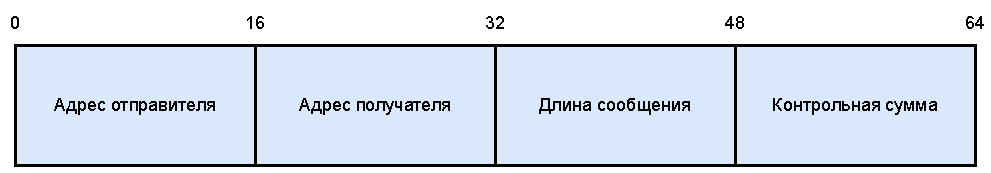
\includegraphics[width=\textwidth]{img/header.pdf}
	\caption{Метаданные пакета}
	\label{fig:header}
\end{figure}

\begin{itemize}
	\item [---] В первых 16-ти битах хранится адрес отправителя пакета.
	\item [---] Биты с 16 по 31 содержат адрес получателя.
	\item [---] Биты с 32 по 47 -- размер зашифрованных данных.
	\item [---] Биты с 48 по 63 -- контрольная сумма пакета.
\end{itemize}

\pagebreak